\documentclass{article}

\title{Novel Project Report: \\ Charge Transport and Mobility in Organic Semiconductors}

\author{Pranay Venkatesh \\ 2019B2A11004P}


\usepackage{graphicx}

\usepackage{hyperref}

\usepackage{listings}

\lstset{
  basicstyle=\ttfamily,
  columns=fullflexible,
  frame=single,
  breaklines=true,
  postbreak=\mbox{\textcolor{red}{$\hookrightarrow$}\space},
}




\hypersetup{
    colorlinks=true,
    linkcolor=blue,
    filecolor=magenta,      
    urlcolor=cyan,
    pdftitle={NP Report},
}


\begin{document}

\begin{titlepage}
   \begin{center}
       \vspace*{1cm}

       \textbf{Charge Transport and Mobility in Organic Semiconductors}
            
       \vspace{1.5cm}

       \textbf{Pranay Venkatesh \\ 2019B2A11004P}

       \vspace{4cm}
            
       A report presented for the course\\
       Novel Project (NP)
            
       \vspace{0.8cm}
     
       
\includegraphics[width=0.3\textwidth]{university}
            
       Department of Chemical Engineering\\
       BITS Pilani, Pilani Campus\\
       Rajasthan\\
       May, 2023
            
   \end{center}
\end{titlepage}


\tableofcontents

\pagebreak


\section{Introduction and Background}

In this report, we will discuss a method we can employ to determine the mobility of charge carriers (electrons and holes) in organic semiconductor materials. Before that it is helpful to review what organic semiconductors are and why they are useful.

\subsection{Organic Semiconductors}

Organic semiconductors are materials that showcase various semiconducting properties, but unlike silicon or other traditional inorganic semiconductors, are based off of carbon-based molecules and polymers. Due to their significant advantages in processability and flexible nature, they have attracted tremendous attention in the past few decades. Their potential for applications in thin film transistors, organic light emitting diodes (OLEDs), photovoltaics (OPVs) and even memory devices has been explored greatly over the past 10-20 years. %TODO: need references, particularly for memory stuff.

Organic semiconductors operate rather differently from traditional inorganic solid-state devices. $\pi$-conjugated electrons in organic molecules are loosely bound and can hence hop or tunnel between molecular states. When organic molecules or polymers begin to "stack" or form layers and lamellar packed motifs, their $\pi$-conjugated rings come close and allow for significant $\pi$-$\pi$ stacking and this allows for regimes where significant charge transport can occur. However, due to mostly disordered regions, we cannot apply the band theory to understand their electronic structure or charge transport properties (more of this is explored in Section 1.2). Instead of doping, organic molecules are oxidised or reduced to introduce carriers and change the nature of the semiconductor material to n or p type accordingly.

Organic semiconductors have various advantages, including low-cost processability, flexibility, a variety of optical properties and compatibility with the environment. Hence they are beginning to dominate the space of research in semiconductor materials.

Since organic materials can interact with a variety of analytes, they have shown promise for gas sensing applications. Several organic molecules change their electrical properties when exposed to specific gases. Hence a macromolecule with one end serving as a binding site and another end serving as an electron transport site acts as a perfect gas sensor. For gas sensing applications, organic molecules have incredible advantages including low-power consumption, high sensitivity and selectivity and quick response time. 

In this report, one particular candidate molecule, BBL (polybenzimidazobenzophenanthroline) is explored for gas sensing applications.

\subsection{Challenge of determining mobility}

Determining the mobility of charge carriers in materials that do not have long-range crystalline order is rather difficult. They do not obey traditional properties of transport and quantum mechanical effects start to dominate.

Given the disordered nature of the material and the fact that quantum effects dominate, we can no longer use convenient methods such as band structure theory or semiclassical transport equations. The movement and mobility of electrons and holes is no longer simply a function of an excitation from a valence band to a conduction band. To compute mobilities of electrons, we now need to consider how they "hop" from site to site. When we have a bunch of molecules bundled up together, these "sites" are basically the HOMO and LUMO levels of the donor and acceptor of the electron in a given hop.


\begin{figure}

    \centering
    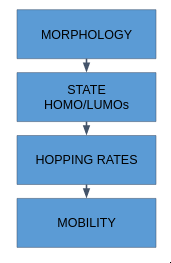
\includegraphics[scale=0.8]{fig1}

\end{figure}


One of the major challenges is to figure out which path an electron will take when it's at any given site. An electron at a given site has many available sites it can hop to. Each of those sites has some hopping likelihood associated with it. So, now the problem we try to address in this project is: given a morphology of equilibrated molecules, (1) how do we determine the electronic states and compute the HOMO and LUMO levels for each site? (2) how do we determine the likelihood of hopping from one site to another? , (3) with all hopping rates, how do we determine the mobility of electrons across the bulk of the material?

The first question is answered in Section 2, where we showcase using semiempirical quantum mechanical methods to solve the Schrodinger equation and obtain the states.

Addressing the second question, many kinetic models have been developed to try and figure out the hopping rates between two quantum states. The model we use here is the semi-classical Marcus model for hopping rates in a two state quantum system, as described in Section 3. To answer the third question: for taking an aggregate of all the hops for all the electrons, we need to run some probabilistic simulation for our system. Here, we use kinetic monte carlo simulations as described in Section 4.


\section{Quantum Chemical Calculations}

% TODO : Cite PySCF, MINDO3.

To get the hopping rates from site to site, it's important to first have the energy changes associated with the hop. This requires us to have information about the electronic structure of each molecule in the system. Specifically, if an electron is hopping from site $i$ to site $j$, we need to have information about the HOMO of site $i$ and the LUMO of site $j$ since we assume the hop takes place as a HOMO to LUMO transition from $i$ to $j$. 

\begin{figure}
    \centering
    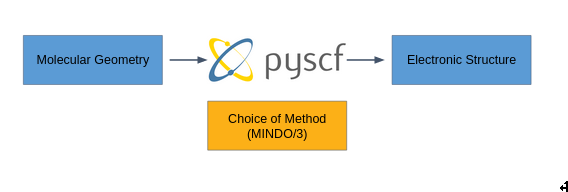
\includegraphics[scale=0.7]{fig2}
\end{figure}


There are many methods we can use to determine the electronic structure of a set of molecules in a morphology, such as Density Functional Theory (DFT). In this case, we apply Semi-Empirical methods, specifically Intermediate Neglect of Differential Overlap (INDO) methods. In our work, the quantum chemical calculations are performed with the MINDO/3 calculations implemented in PySCF. Other programs use DFT-based methods, however comparison of INDO-based results have shown good agreement with those performed with DFT calculations. 



\section{Marcus Theory}

% TODO : Cite the original Marcus theory papers(?)

We can model the charge hops between two molecules or sites in an organic semiconductor as a set of nonadiabatic thermally active processes. If we model each site as a parabolic potential well, we need to sample some of the parameters of the intersection of two parabolic site energies to understand the hopping rate.

From the Frank-Condon principle, we can further assume that the morphology of nuclei stays frozen during the electron transport reaction and further that the intersection point corresponds to a unique equilibrium geometry.

\begin{figure}

    \centering
    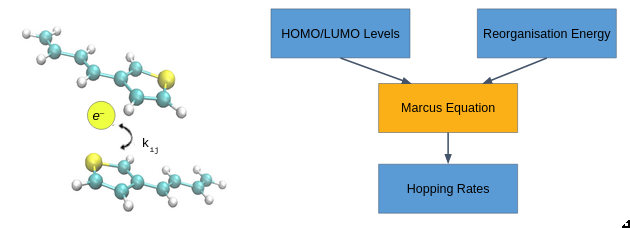
\includegraphics[scale=0.6]{fig3}

\end{figure}

% TODO : add an image of two intersecting parabolas to show Marcus energies like in Jimmy thesis.

Now, an Arrhenius model can be used to model the kinetics of the electron transport reaction between sites. For an electron transport reaction between sites i and j, we can devise a model for the hopping rate $k_{ij}$ using an appropriate exponential Arrhenius equation as such :

$$k_{ij} = \frac{2 \pi |T_{ij}|^2}{\hbar \sqrt{4 \pi \lambda_{ij} k_{B} T}} \exp\left[-\frac{(\Delta E_{ij} - \lambda_{ij})^2}{4 \pi \lambda_{ij} k_{B} T}\right]$$

Here, $T_{ij}$ represents the overlap between the electronic states, $\lambda_{ij}$ is the reorganisation energy of the system and $\Delta E_{ij}$ is the free energy change.

%TODO : Site the reorganisation energy eric paper

The $\lambda_{ij}$ term is important since it exemplifies the semiclassical nature of the Marcus equation. $\lambda_{ij}$ is called the reorganisation energy. It represents the energy required to "reorganise" the electronic states of the system, prior to any charge transferring. $\lambda$ values have to be determined either empirically or using very specific electronic structure methods, beyond the scope of this report. % TODO : Find papers for BBL reorganisation energy and cite.
For the case of BBL polymers, several literature records provide the value of the reorganisation energy, which we can use in the Marcus equation.

The energy value $\Delta E_{ij}$ is given by:

$$\Delta E_{ij} = E_{homo, i} - E_{homo, j}$$

and the overlap $T_{ij}$ can be computed by considering a dimer formed by "overlapping" the pair of sites (forming a dimer) and then comparing the site energy difference when overlapped and when separated:

$$T_{ij} = \frac{1}{2} \sqrt{(E_{homo,dimer} - E_{homo-1,dimer})^2 - (\Delta E_{ij})^2}$$

\section{Kinetic Monte Carlo Model}

%TODO: Cite Voter literature for kMC stuff

The Kinetic Monte Carlo method is a probabilistic method to determine the movement of a system from state to state. In particular, it is useful for a case like ours where the hopping rates ($k_{ij}$) are known and we want to simulate all electron hops to ascertain the mobility of charge carriers.

The probability of an electron hopping from i to j is given by: $$P_{ij} = k_{ij} \exp(-k_{ij} t)$$. 

This probability model is the result of assuming that the hopping reaction is a first order process, i.e. when the system is at state i, it has no "memory" of how it reached the state. Hops are hence modelled here as rare events.

\begin{figure}

    \centering
    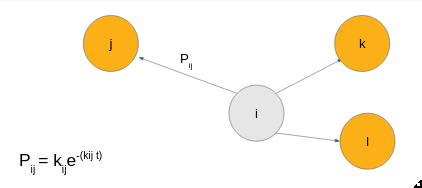
\includegraphics[scale=0.6]{fig4}
\end{figure}

One way of simulating the system's path is to employ the following procedure :

\begin{itemize}
    \item Generate a random number r from a uniform probability distribution in (0, 1).
    \item $r = e^{-kt}$, so we get the drawing time $t_{draw} = -\frac{1}{k} \ln(r)$
    \item Now when the system is in state i, compute all $k_{ij}$ and derive the drawing times $t_{j}$ for hops to each state $j$ by generating random numbers using the procedure prescribed above.
    \item Find which state j provides the minimum $t_j$.
    \item Move the system from i to j.
    \item Repeat.
\end{itemize}

This provides the entire hopping pathway of electrons in the system. Now, if we want to get the mobility, we need to use the Einstein-Smoluchowski relation. The diffusivity of electrons in the system can be derived by using the mean-squared distance of electron hops. From this diffusivity value the mobility can be derived as such :

$$\mu = \frac{q D}{k_B T}$$

\section{Installing and using MorphCT}

%TODO: Cite MorphCT zenodo and Eric paper

MorphCT is the software we use to implement our workflow, since the entire operation can be carried out in Python and it is completely an open source software. 

\subsection{Getting python and conda}

To install MorphCT, first begin by installing python and anaconda. Understanding some of the basics of python, pip and anaconda is very helpful in working with MorphCT. Anaconda can be installed by running the following commands (in Linux / WSL / your Cyclops account) :

\begin{lstlisting}[language=bash]
    curl -sL \
    "https://repo.anaconda.com/miniconda/Miniconda3-latest-Linux-x86_64.sh" \ >
    "Miniconda3.sh"
\end{lstlisting}

This adds the Miniconda3 install script to your home directory. Now install miniconda by running:

\begin{lstlisting}[language=bash]

    bash Miniconda3.sh

\end{lstlisting}

\subsection{Install MorphCT}

Get the morphCT files to your home directory by using the following command (make sure you have git installed) :

\begin{lstlisting}[language=bash]

git clone https://github.com/cmelab/morphct.git

\end{lstlisting}

Go into the MorphCT directory and create a conda environment for installing the package:

\begin{lstlisting}[language=bash]

cd morphct

conda env create -f environment.yml

\end{lstlisting}

This will take some time, but it will set up the requirements for morphct. Now, complete the installation for morphct:

\begin{lstlisting}[language=bash]

conda activate morphct

pip install -e .

\end{lstlisting}

The "." at the end of the command is important, since it specifies that you want to install it in that directory. This should complete the installation of morphct.

Now, while in the morphct environment, you can run python scripts and programs that utilise morphct or its dependencies.

\section{LAMMPS-to-Mobility Workflow}

LAMMPS is not a python-based software nor is it traditionally compatible with the python toolkits that we are using for MorphCT.

Hence for working with MorphCT, we need to convert the LAMMPS morphology into an appropriate file to use it. I have created a workflow to take a snapshot of a LAMMPS molecular dynamics (MD) simulation output. The workflow I developed is described in the package : \href{https://github.com/chemicalfiend/lammps-carrier-mobility}{lammps-carrier-mobility}

To use this workflow, start by extracting the coordinate and bond data into separate files called "sorted\_coords.data" and "sorted\_bonds.data". The data should be sorted by atom number and bond number. To run MorphCT,we need to convert the LAMMPS data files of the morphology into gsd files. To convert files into gsd files, we can use the mbuild package, which can save atoms and molecules as gsd files. The script gsdwriter.py converts the sorted coordinates and sorted bonds files into a gsd file. 

\begin{lstlisting}[language=python]

"""

Program to write a GSD file for a trajectory from a LAMMPS data file.

Used for Charge Transport calculations

"""


import mbuild as mb
import numpy as np
import os

num_molecules = 10
atoms_per_mol = 158


if(os.path.exists("system.gsd")):
    os.remove("system.gsd")
class Atom:
    def __init__(self, n, mol, typeid, charge, x, y, z):
        self.n = n
        self.mol = mol
        self.charge = charge
        self.x = x
        self.y = y
        self.z = z

        if(typeid <= 18):
            self.atomtype = "C"

        elif(typeid > 18 and typeid <= 31):
            self.atomtype = "H"

        elif(typeid == 32):
            self.atomtype = "F"
        
        elif(typeid == 33):
            self.atomtype = "Cl"

        elif(typeid == 34):
            self.atomtype = "Br"

        elif(typeid == 35):
            self.atomtype = "I"

        elif(typeid >= 36 and typeid <= 56):
            self.atomtype = "N"

        elif(typeid >= 57 and typeid <= 62):
            self.atomtype = "O"

        elif (typeid >= 63 and typeid <= 73):
            self.atomtype = "P"

        elif (typeid >= 74 and typeid <= 83):
            self.atomtype = "S"

        else:
            self.atomtype = " "

class Bond:
    def __init__(self, a1, a2):
        self.atom1 = a1
        self.atom2 = a2


fc = open("sorted_coords.data", "r")
fb = open("sorted_bonds.data", "r")

clines = fc.readlines()
blines = fb.readlines()

atoms = []


for line in clines:
    tokens = line.split()
    #print(tokens)    
    n = int(tokens[0])
    mol = int(tokens[1])
    typeid = int(tokens[2])
    charge = float(tokens[3])
    x = float(tokens[4])
    y = float(tokens[5])
    z = float(tokens[6])
    
    atoms.append(Atom(n, mol, typeid, charge, x, y, z))

# Store and add bonds


bondi = []
bondj = []

for line in blines:
    tokens = line.split()
    #print(tokens)
    atom1 = int(tokens[2])
    atom2 = int(tokens[3])

    bondi.append(atom1)
    bondj.append(atom2)

#print(bondi)
#print(bondj)
system = mb.Compound()

# System box and other parameters set.

#system.box = mb.Box([xhi-xlo, yhi-ylo, zhi-zlo])

for i in range(num_molecules):
    m = i + 1
    mol = mb.Compound()

    for atom in atoms:
        if atom.mol == m:
            a = mb.Particle(pos=[atom.x, atom.y, atom.z], element = atom.atomtype, name=atom.atomtype, charge= atom.charge)
            mol.add(a)

    system.add(mol)

"""
for atom in atoms:
    a = mb.Particle(pos=[atom.x, atom.y, atom.z], element = atom.atomtype, name=atom.atomtype, charge= atom.charge)
    system.add(a)
"""
for i in range(len(bondi)):
    system.add_bond((system[bondi[i] - 1], system[bondj[i] - 1]))


print(system.n_bonds)

system.save("system.gsd")


\end{lstlisting}

To run the script gsdwriter.py, we first require the mbuild and gsd packages. In your conda environment, use the following command to install mbuild :

\begin{lstlisting}[language=bash]

conda install -c conda-forge mbuild

conda install -c conda-forge gsd

\end{lstlisting}

Now, we can run the script by running:

\begin{lstlisting}[language=bash]

python3 gsdwriter.py

\end{lstlisting}


Running the script takes time. It generates the output file : "system.gsd", for which we can perform the Kinetic Monte Carlo analysis.

The script "kmc-analysis.py" lays out a basic template for calculating the mobility of the system with MorphCT. To run this script, the MorphCT environment must be activated.

\subsubsection*{Surprising Revelation}

The mbuild function "add\_bond" which was used as a part of the gsdwriter script turned out to be a very slow function. In an effort to improve the performance of this function, I submitted an issue to the mbuild github repository.

\section{Results and Discussion}

\subsection{10 Molecules Test System}

To test the working of the workflow, the mobility calculations were performed on a morphology of 10 PEDOT molecules. The calculations were performed as prescribed in the script "kmc-script.py" specified in the lammps-carrier-mobility, as mentioned previously. 

First, a LAMMPS simulation was carried out for equilibrating 10 PEDOT molecules in vacuum. The output was dumped as a LAMMPS data file. The coordinates and bonds were then extracted for using the GSD conversion workflow.

The MINDO/3 calculations on each molecule were computed in PySCF and the kMC calculations were performed by the MorphCT software. This determines the charge carrier mobility of the system.

\begin{figure}
    \centering
    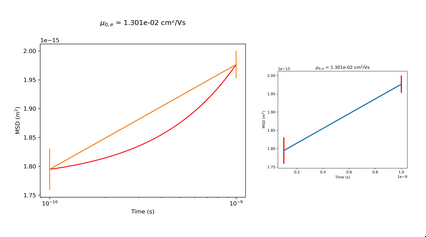
\includegraphics[scale=0.6]{fig5}
\end{figure}


%TODO: add the analysis images from MorphCT output


%TODO : add Bibliography with bibtex

\end{document}



